% REMEMBER: You must not plagiarise anything in your report. Be extremely careful.

\documentclass{l4proj}

    
%
% put any additional packages here
%

\begin{document}

%==============================================================================
%% METADATA
\title{A Sailing Race Manager}
\author{Hamish Philip}
\date{March 24, 2023}

\maketitle

%==============================================================================
%% ABSTRACT
\begin{abstract}
    TODO
\end{abstract}

%==============================================================================

% EDUCATION REUSE CONSENT FORM
% If you consent to your project being shown to future students for educational purposes
% then insert your name and the date below to  sign the education use form that appears in the front of the document. 
% You must explicitly give consent if you wish to do so.
% If you sign, your project may be included in the Hall of Fame if it scores particularly highly.
%
% Please note that you are under no obligation to sign 
% this declaration, but doing so would help future students.
%
\def\consentname {Hamish Philip} % your full name
\def\consentdate {March 24, 2023} % the date you agree
%
\educationalconsent


%==============================================================================
\tableofcontents

%==============================================================================
%% Notes on formatting
%==============================================================================
% The first page, abstract and table of contents are numbered using Roman numerals and are not
% included in the page count. 
%
% From now on pages are numbered
% using Arabic numerals. Therefore, immediately after the first call to \chapter we need the call
% \pagenumbering{arabic} and this should be called once only in the document. 
%
% Do not alter the bibliography style.
%
% The first Chapter should then be on page 1. You are allowed 40 pages for a 40 credit project and 30 pages for a 
% 20 credit report. This includes everything numbered in Arabic numerals (excluding front matter) up
% to but excluding the appendices and bibliography.
%
% You must not alter text size (it is currently 10pt) or alter margins or spacing.
%
%
%==================================================================================================================================
%
% IMPORTANT
% The chapter headings here are **suggestions**. You don't have to follow this model if
% it doesn't fit your project. Every project should have an introduction and conclusion,
% however. 
%
%==================================================================================================================================
\chapter{Introduction}

% reset page numbering. Don't remove this!
\pagenumbering{arabic} 

In the UK, sailing races are scored with rules set by the Royal Yachting Association (RYA).
This scoring method results in many calculations which can be tedious to do by hand. As a result of this, most scoring is done using computer systems \citep{RYAscore}.

\begin{figure}[h!]
    \centering
    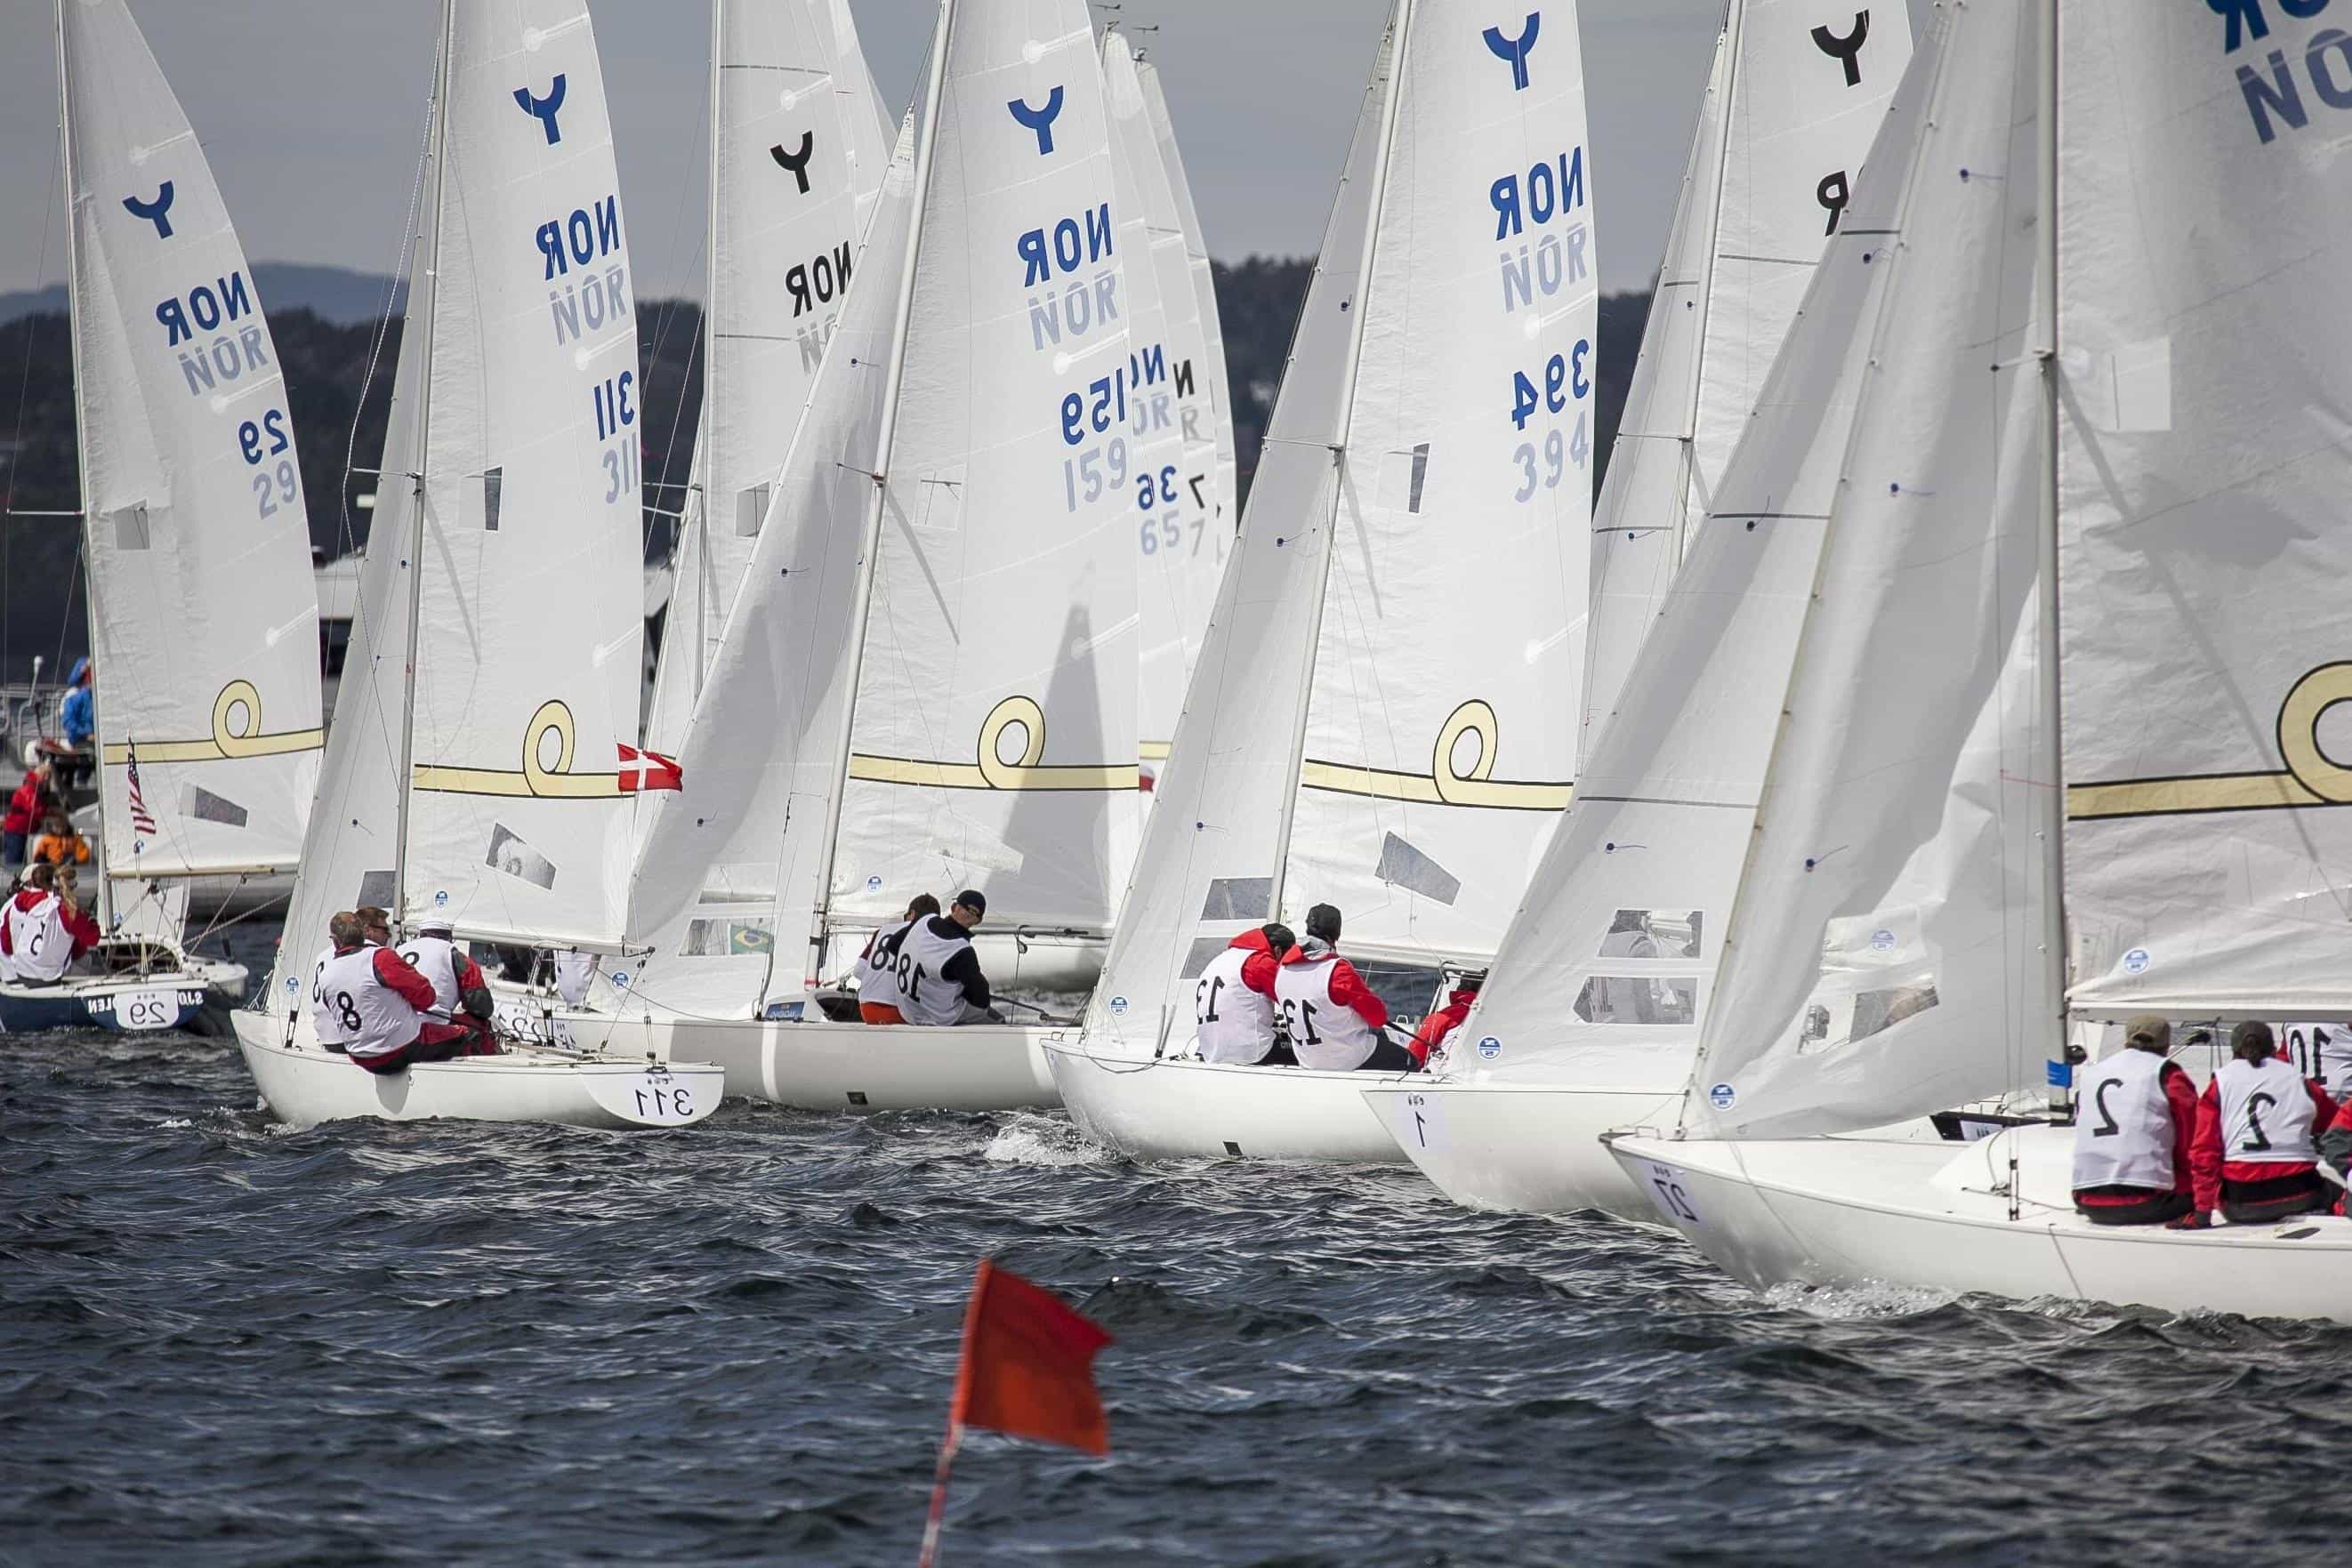
\includegraphics[width=0.6\linewidth]{images/SailingRace.jpg} 

    \caption{A Dingy Sailing Race \citep{SailingRace}
    }

    % use the notation fig:name to cross reference a figure
    \label{fig:SailingRace} 
\end{figure}

Castle Semple Sailing Club on Lochwinnoch, Scotland, currently uses a desktop application called Sailwave to score their races. This app has many issues, and the club desires a better system. The goal of this project is to design and build an improved system, that the sailing club can use to replace their current one \citep{RYAscore}.

Castle Semple Sailing Club on Lochwinnoch, Scotland, currently uses a desktop application called Sailwave to score their races. This app has many issues, and the club desires a better system. The goal of this project is to design and build an improved system, that the sailing club can use to replace their current one.

\section{The Client}
The Client for this project is Castle Semple Sailing Club. Located on Lochwinnoch near Glasgow, Scotland, It hosts many races and events throughout the year and uses a variety of different classes of dinghy. The majority of Castle Semple Sailing Club members have limited computer skills. Which needs to be taken into account when designing the solution.

The main point of contact with the club is Dr Simon Rogers, a member of the Castle Semple Sailing Club Committee. He was previously a lecturer at the School of Computing Science at the University of Glasgow, and so he has technical knowledge that is relevant to the project. However, he is not able to spare the time to be directly involved in the project, so interaction with him is limited.

\section{The Problem}
According to the \citet{RYAscore} website, the scoring rules to be used in sailing races, described in high level terms, consists of the following:

A sailor receives points based on their finishing position (1 points for 1st, 2 points for 2nd etc.). The sailor with the lowest number of points as the end of a series (a collection of races) wins that series. Their place in the race is determined by the time they took to completed it, which is corrected by a handicap, so sailors in different boats with different capabilities can race fairly. These handicaps are set by the RYA, and in the case of dingy sailing, are known as the Portsmouth Yardstick Scheme
\citep{RYApy}

Additionally, a sailor can choose to not participate in any number of races in a series, in which case they are awarded a number of points that is greater than those any sailor who did compete received. A sailor can also start, but not finish, a race, in which case they are awarded a slightly smaller number of points than not participating. Finally, a sailor can also be involved in running the race, in which case they are given a medium amount of points to reflect their contribution.

The current software, Sailwave, that the sailing club uses has a few limitations. Firstly, as it is a desktop program, it is limited to use on a computer that is owned by the club. This computer is old and slow, resulting in poor performance of the program, and cannot be easily replaced.

\begin{figure}[h!]
    \centering
    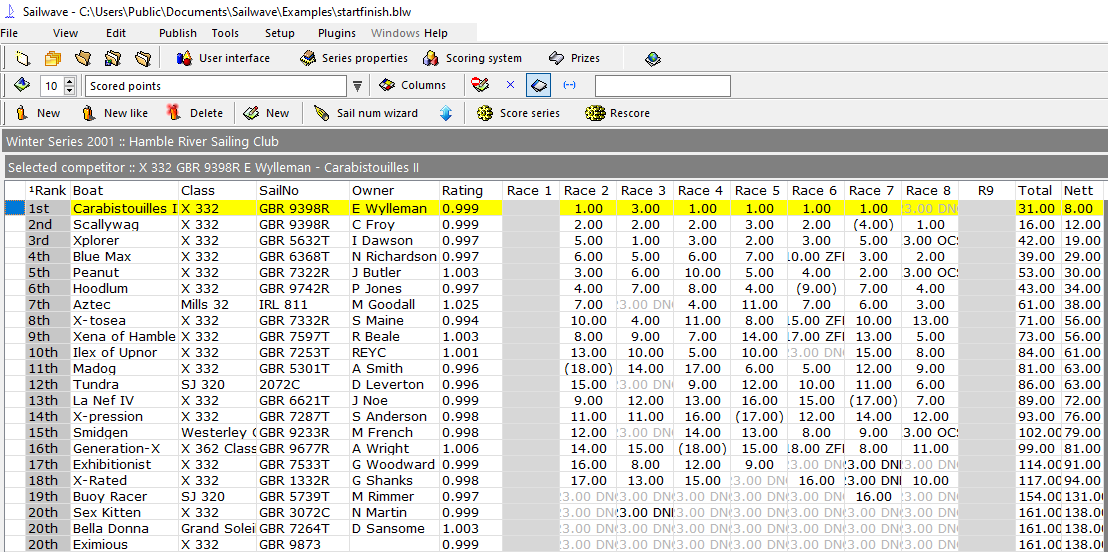
\includegraphics[width=0.6\linewidth]{images/Sailwave.png} 

    \caption{Main screen of the Sailwave Program \citep{sailwave}
    }

    % use the notation fig:name to cross reference a figure
    \label{fig:Sailwave} 
\end{figure}

Additionally, the software itself is outdated and clunky, having been originally made in 2001 \citep{sailwave}. This can be seen in figure \ref{fig:Sailwave}, which shows the main screen of the Sailwave program. Notice how it is cluttered and confusing. 

In order to distribute the results of a race or series to the sailors, the results need to be printed out and manually sent out via another channel, such as email or posting the results on a notice board. This is not ideal. Also, the users of the software at Castle Semple Sailing Club have limited computer skills, so updating the program, moving the program to a new pc or selecting a new program to use is difficult.

This project sets out to design a new sailing race managing system, that solves the problem of calculating a leader board from data collected from races, using the system specified by the RYA. The system must improve upon Sailwave, and that provides some other features that the Castle Semple Sailing Club desires.


%==================================================================================================================================
\chapter{Background}\label{chap:Back}
This section will explore the background information 
the problem.

\section{Sail Racing}
The official rules for sailing races, known as The Racing Rules of Sailing, are set out, and updated every 4 years, by World Sailing, the international authority for the sport. Curtain deviations from these rules are allowed to be made by Member National Authorities, which for the UK, is the Royal Yachting Association (RYA). The RYA published these rules in a document called RYA Racing Rules Guidance \citep{RYAscore}.

In general, a sailing race works by participants sailing round a set course. This can be small as in a dingy race, or go all the way around the world, such as in the Golden Globe Race. The time they take to sail around the course is measured. This time is then adjusted with what is known as a handicap, which accounts for the different sailing abilities of different boats. The boat that took the shortest time, corrected by the handicap, wins.

The RYA provides guidance as to how a sailing race should be scored. This Guidance is based on the rules set out by World Sailing. It is up to the committee organising the race as to which scoring system is used. The recommended and default system to use is the “Low Points System”.

The low points system works by granting the participant in 1st place, with the lowest corrected time, 1 point, the one in second place 2 points etc. Participants can also we awarded a variety of different penalty points in various circumstances, for example not competing in a race, or starting but not finishing. The full set of circumstances and the associated points are specified in the RYA racing rules guidance document \citet{RYAscore}.

Multiple races form a series, often a tournament in other sports. The participants points from all the races in the series are added together, and the one with the lowest number of points wins. In this way, a participant need not compete in every race in a series in order to take part, but for every race they do not compete in, their score will increase due to the penalty points.

Handicaps, how they work, their history and how they are calculated are explained in the paper “Sailing close to the statistics” \citep{hanicaps}. Wolstenholme says that Handicaps allow boats with different capabilities to race against each other fairly, sparing the performance of the boat from the performance of the crew. 
According to \citet{hanicaps}, a common handicap method is a time-on-time approach. This is where a time correction is applied to a boat’s finishing time. This is the method recommended by the RYA.

The exact method generally used in dingy sailing in the UK is the Portsmouth Yardstick Scheme, which was created in 1951 \citep{hanicaps}. In this system, handicaps are given as a number close to 1000. An extract from the Portsmouth Yardstick Scheme Number list \citep{RYApy} can be seen in figure \ref{fig:Hanicaps}

To use the handicaps from provided by the scheme to calculate a corrected time, The following formula is applied to the time in seconds:

\begin{equation}
    \text{Corrected Time(seconds)} = \frac{\text{Time(seconds)} \times 1000}{\text{Handicap}},
    \label{eq:1}
\end{equation}  

This formula means handicap values under 1000 increase the time, thus slowing boats down, and those over 1000 reduce it, thus speeding boats up. The result is the corrected time in seconds, which is used in scoring \citep{RYAscore}.

\begin{figure}[h!]
    \centering
    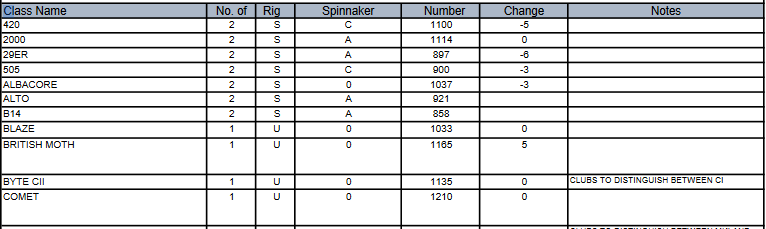
\includegraphics[width=0.6\linewidth]{images/Handicaps.png} 

    \caption{Extract from the Portsmouth Yardstick Scheme handicap number list \citep{RYApy}
    }

    % use the notation fig:name to cross reference a figure
    \label{fig:Hanicaps} 
\end{figure}

Historicity, handicaps have been calculated either using past performance, or on the physical design of the boat. The Portsmouth Yardstick scheme updates their handicaps based on past club race results, and updates them every year \citep{hanicaps}.

\section{Scoring systems}
The underling problem to a sailing race manager is simply a system that records and displayed results. Many of these exist across many different sports. By looking at some of these systems, we can get an idea about what makes a scoring system, that can be used to inform this project.

One example is part of the website of the Lawn tennis association \citet{Tennis} which displays the results of tennis torments. A screenshot from the website is pictured in figure \ref{fig:Tennis} below.

\begin{figure}[h!]
    \centering
    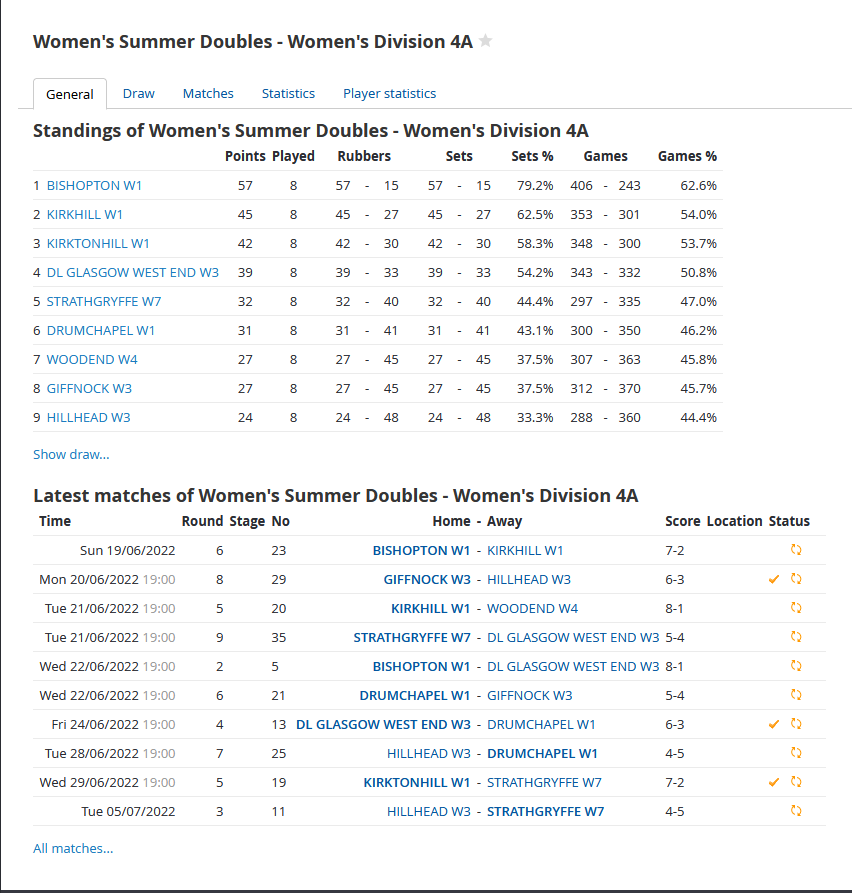
\includegraphics[width=0.6\linewidth]{images/Tennis systme.png} 

    \caption{results page of LTA Women's Summer Doubles \citep{Tennis}
    }

    % use the notation fig:name to cross reference a figure
    \label{fig:Tennis} 
\end{figure}

It can be seen that the page consists of a table, listing the participants in the order of who is winning, along with some score statistics. This is a simple formula that most scoring systems seem to follow.

Another example is the results page on the website of the Victoria Park Run, Glasgow, which is shown below in figure \ref{fig:parkrun}.

\begin{figure}[h!]
    \centering
    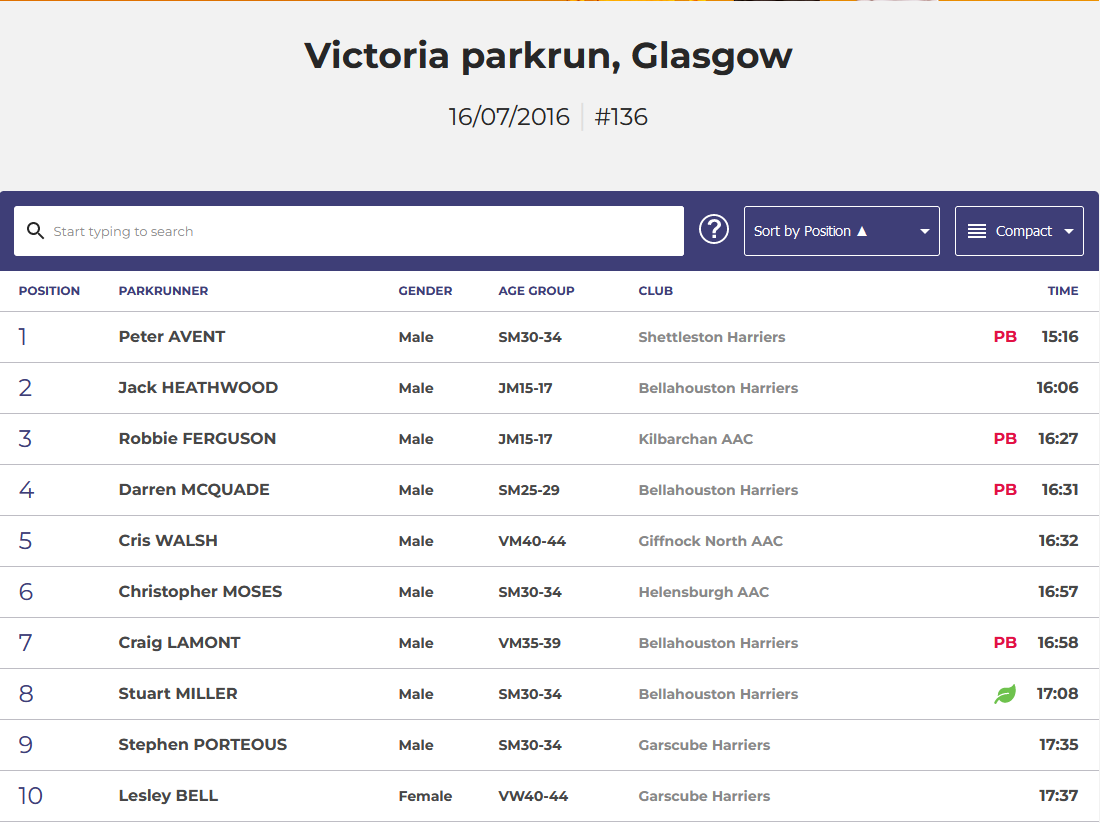
\includegraphics[width=0.6\linewidth]{images/ParkRun.png} 

    \caption{results page of the Victoria Park Run, Glasgow \citep{Parkrun}
    }

    % use the notation fig:name to cross reference a figure
    \label{fig:parkrun} 
\end{figure}

This results page looks much the same as that from the Lawn tennis association \citet{Tennis}. List of participants, ordered by who is winning, with some relevant statistics. The part of this project that involves displaying the results is conceptually similar to these two examples.

The previous two examples are just results pages, where this project is also concerned with a system to calculate those results. A closer example to this project can be found in a dissertation by Ying Lu \citet{Multi-sport} which developed a system to manage multi-sport events, such as a triathlon. It resulted in a system that could organize different races, and calculate and display results. This is a similar problem to that this project is trying to solve.

\section{Currently existing Sailing race Management systems}
Diving more deeply into scoring systems in the context of sail racing, a number of systems already exist. These can be drawn on for inspiration.

The most obvious one is the system the client currently uses: Sailwave \citet{sailwave}. Sailwave is free, but closed source, software, originally released in 2001. It enables the inputting, calculating and output of Sailing race results, and comes with a large amount of other features. A new system that is close to that Castle Semple Sailing Club already use, but that improves upon it, is likely to be successful. 

An additional system is Sailing Club Manager \citet{ClubManager}, which is a system for managing everything to do with a sailing club, from race scoring to member fees. It has a much wider scope than this project, but still implements the same features, and so it still useful.

Finally, Sail event \citet{SailEvent} is a web-based system for sailing race management. It takes a different approach the Sailwave, being entirely web-based and has a distinctly different user interface.

Detailed analysis of these three systems to inform the requirements for this project is done in the next chapter \autoref{chap:A/R}.




%==================================================================================================================================
\chapter{Analysis/Requirements}\label{chap:A/R}
\section{Analysis of Current solutions}
This section will take a dive into three currently existing sailing race management systems, and identify what can be learned from how they approached this problem.
\subsection{Sailwave}
Sailwave \citet{sailwave} is the software currently used by Castle Semple Sailing Club. It is free, but closed source, software, originally released in 2001.
The front page of its website \citep{sailwave} states: “Sailwave is a popular, fully-featured, easy-to-use, multilingual, sailing results/scoring application for Windows from XP to Windows 11“

Sailwave has a large list of features. Some notable ones, also taken from the front page of its website \citep{sailwave} are as follows:
\begin{itemize}
    \item
    Flexible scoring: score across all competitors or by fleet, club, nationality, etc.
    \item
    Publish retirement sheets, competitor lists, alternative penalty sheets, etc.
    \item
    Send your news (reports, results, and photos) directly to the Yachts and Yachting magazine website.
    \item
    Publish directly into programs like Microsoft Word and Excel etc,
    \item
    Publish to web documents (HTML) for upload to websites or printing or emailing. Integrated support for FTP/SFTP/SSH/FTPS.
\end{itemize}

It can be seen that the software contains a myriad of different features and use cases. The front page of its website lists 33 different features, some of which were shown above. It can be deduced from this that the program is bloated, cluttered and confusing.
Figure \ref{fig:SailwaveEmpty} shows the page a user is greeted with upon first startup of the program. There are many bottoms and menus presented in the tool bar, but many are greyed out and it is not immediately clear where to start.

\begin{figure}[h!]
    \centering
    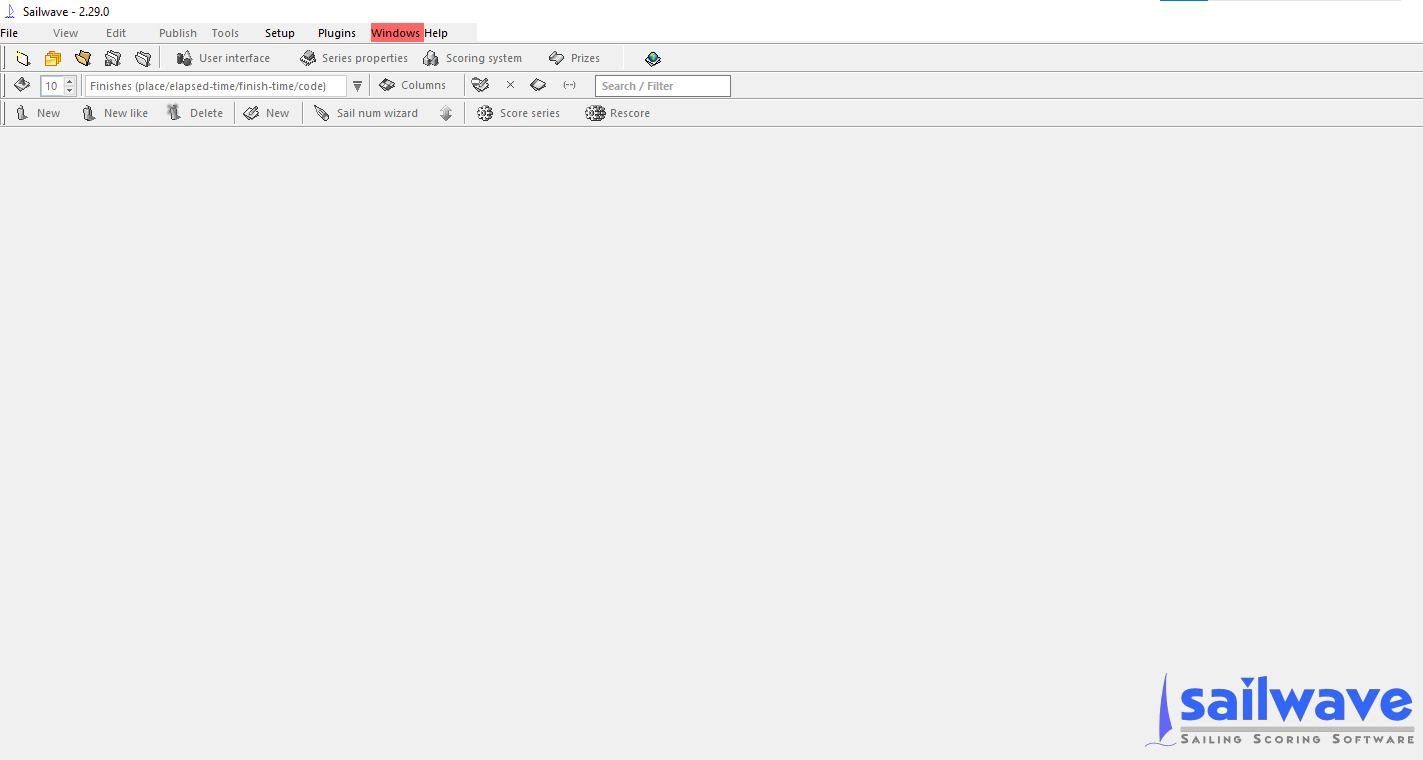
\includegraphics[width=0.6\linewidth]{images/SailwaveEmpty.png} 

    \caption{Start-up screen of the Sailwave program \citep{sailwave}
    }

    % use the notation fig:name to cross reference a figure
    \label{fig:SailwaveEmpty} 
\end{figure}

Figure \ref{fig:SailwaveEdit} shows Sailwave when a user has started a new series and is attempting to edit one of the entries. A massive amount of different fields are available to be filled out across multiple tabs. It is not clear which cell in the excel-like table corresponds with which entry in the dialogue box. It is clear that Sailwave provides lots of support for various uses, but how much of what Sailwave does it directly relevant to a small sailing club? The importance of restricting the features of programs is shown in an article by \citet{leanSoftware}. In it, he says that bloated software takes more time to design, code and debug. This can be seen in Sailwave, as to reach its current state, the software has been continually added to over the past 22-years, since its first release in 2001 \citep{sailwave}.

\begin{figure}[h!]
    \centering
    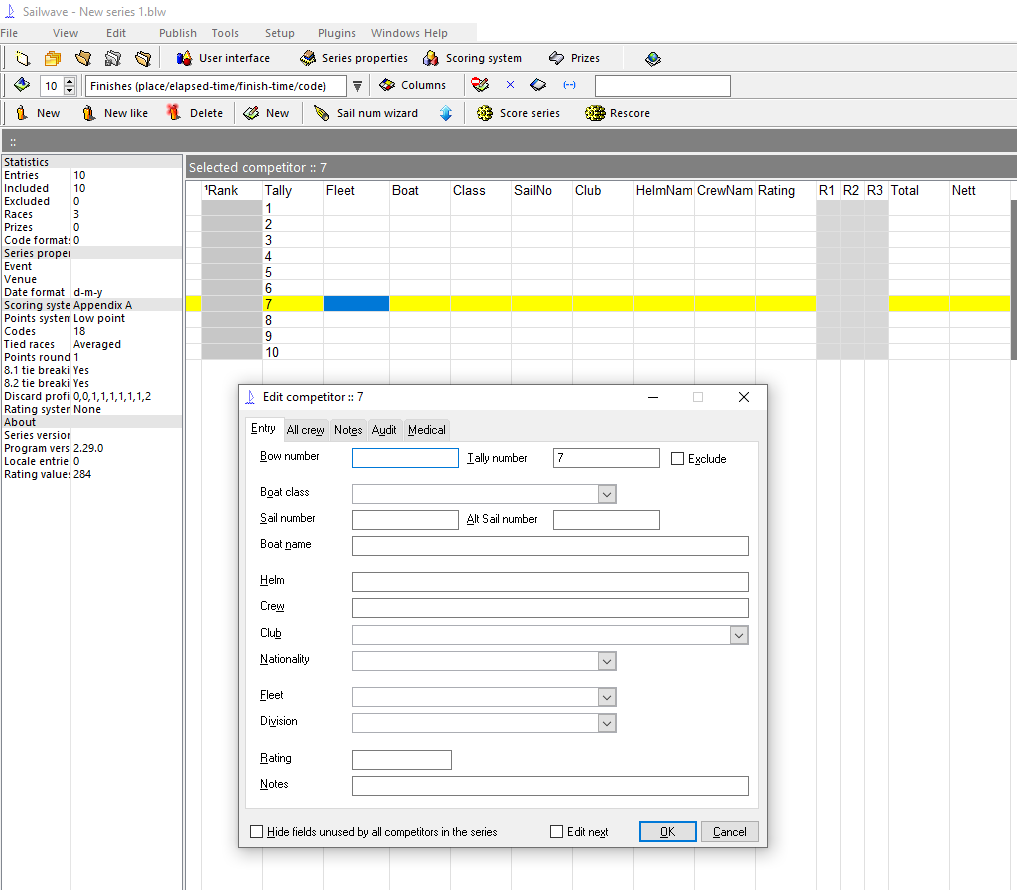
\includegraphics[width=0.6\linewidth]{images/Sailwave_edit.png} 

    \caption{Editing a cell in the Sailwave Program \citep{sailwave}
    }

    % use the notation fig:name to cross reference a figure
    \label{fig:SailwaveEdit} 
\end{figure}

Sailwave does succeed in presenting some of its information, mainly the race details shown in the excel-like table as can be seen in figure \ref{fig:Sailwave}, in a clear and easy to understand manner. The format of the data takes after a Microsoft Excel spreadsheet \citep{Excel}, shown in figure \ref{fig:Excel}, The resemblance is apparent. As many people are familiar with spreadsheets, past skills can make it more easy for a users to understand Sailwave.

\begin{figure}[h!]
    \centering
    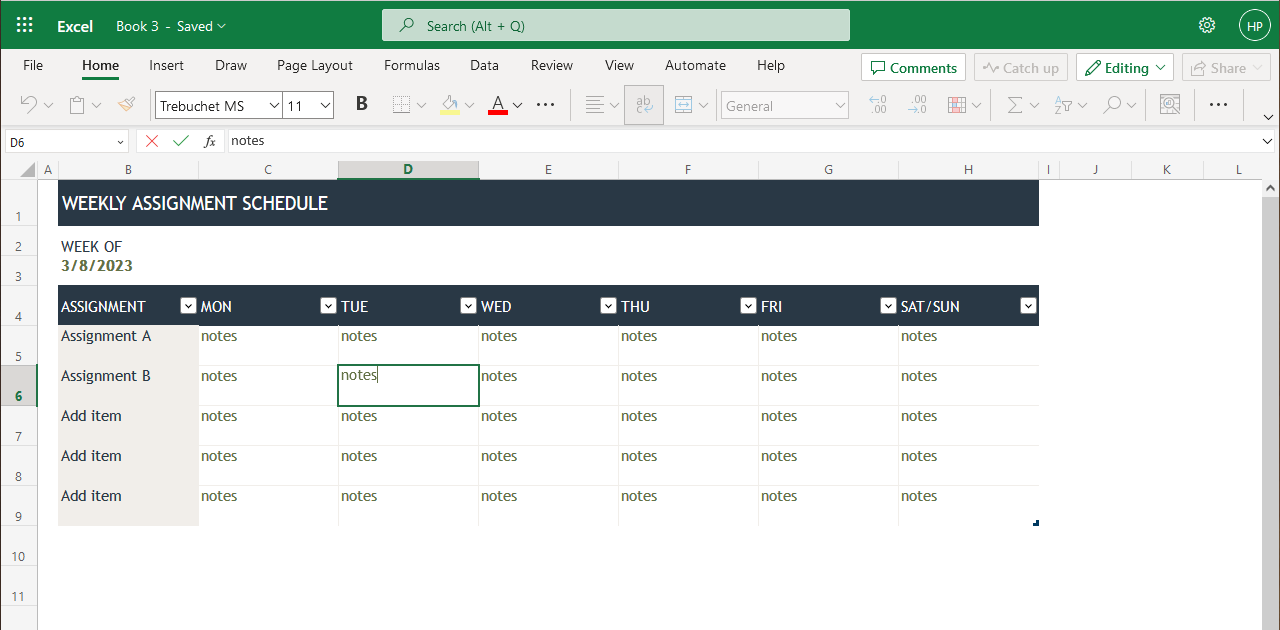
\includegraphics[width=0.6\linewidth]{images/Ecel.png} 

    \caption{Example of a common Excel spreadsheet \citep{Excel}
    }

    % use the notation fig:name to cross reference a figure
    \label{fig:Excel} 
\end{figure}

Overall, the standardised excel-like format Sailwave uses is a good lesson that can be learned from when designing a new solution, particularly as the members of Castle Semple Sailing Club are already used to Sailwave. The over-complexity and feature-bloat of Sailwave presents an opportunity to improve upon it, by cutting out many of the features that aren't relevant to a small-scale sailing club.

\subsection{Club manager}
\citet{ClubManager} is a web-based application that takes different approach. It seeks to provide a complete platform to manager every part of a sailing club, from race scoring to membership management to morning booking. It is purchased via a subscription. 
While the scope of club manager is obviously far beyond the problem this project seeks to tackle, it does show an example of a more professional solution. As Sailing Club Manager is paid software, and the don’t provide any example on their website, the exact functionality of it cannot be analysed and compared.
Focusing in on the race scoring feature, the website \citep{ClubManager}, shown in figure \ref{fig:ClubManager},  lists, among others, the following features:

\begin{itemize}
    \item
    Flexible scoring: score across all competitors or by fleet, club, nationality, etc.
    \item
    It can be used on any device that can browse the internet including tablets, Macs and PCs. 
    \item
    It's easy to use and doesn't require Race officers to learn complicated software. 
\end{itemize}

\begin{figure}[h!]
    \centering
    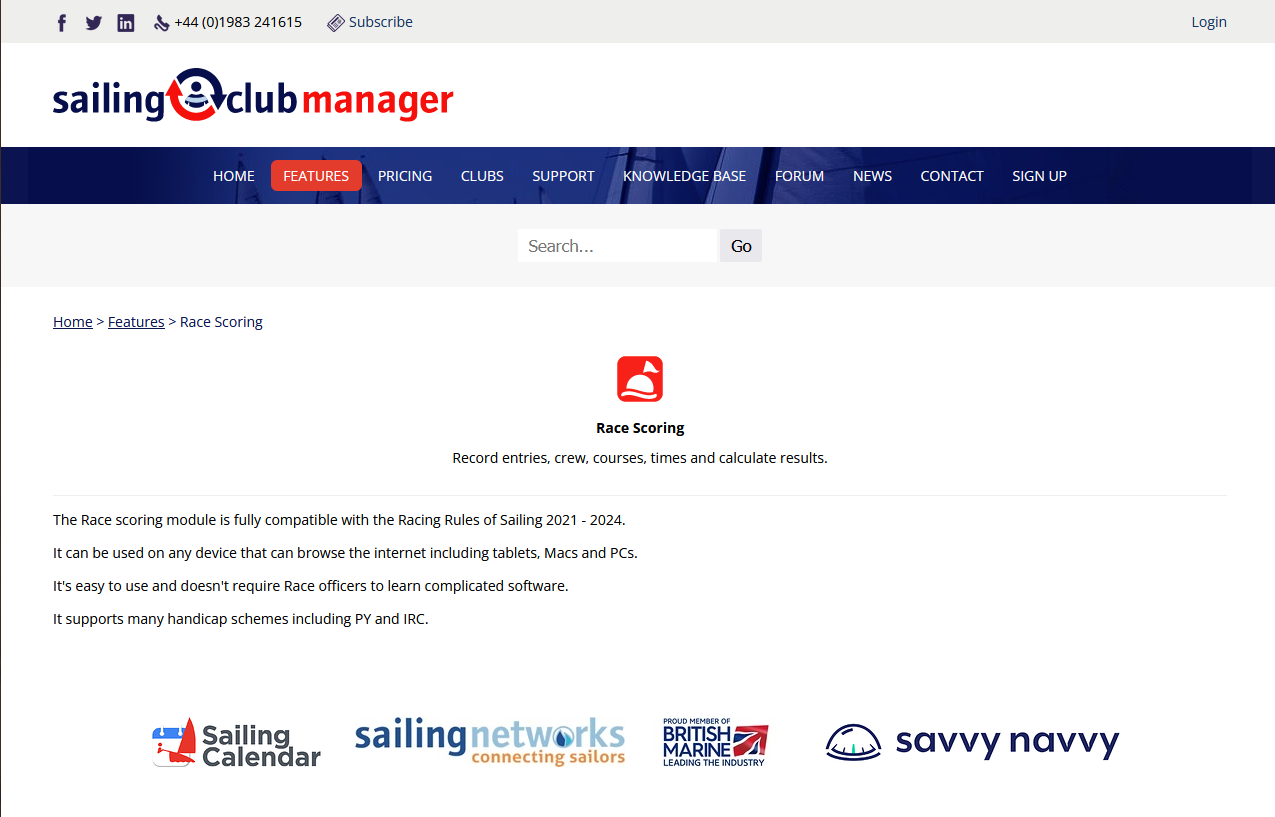
\includegraphics[width=0.6\linewidth]{images/ClubManager.png} 

    \caption{Race scoring Features page on the Sailing Club Manager Website \citep{ClubManager}
    }

    % use the notation fig:name to cross reference a figure
    \label{fig:ClubManager}
\end{figure}
Compared to Sailwave, the features are much smaller in number, and directed towards a simple use-case, Rather than the sheer density of features Sailwave provides. This shows that this software is much more directed towards ease of use and practicality, than Sailwave. Due to the lack of tech skills among the members of Castle Semple Sailing Club, having a new solution take an approach more similar to club manager may be beneficial.

As the scope of Sailing Club Manager far exceeds that of what Castle Semple Sailing Club want, it can be used as an example of what to stay away from. If the scope and features of a new solution begin to resemble that of Sailing Club Manager, then they should be reduced.


\subsection{Sail Event}

Sail Event \citet{SailEvent} is a web-based application that is very similar to Sailwave in what it does. However, it does so in a very different way. It is again a free, but closed source, web-app, with a paid version that provides more features. Users can log in as either a club or a sailor. Clubs can create races, sailors can join them. A screenshot of the user interface where races are created is shown in figure \ref{fig:sailEvent}

\begin{figure}[h!]
    \centering
    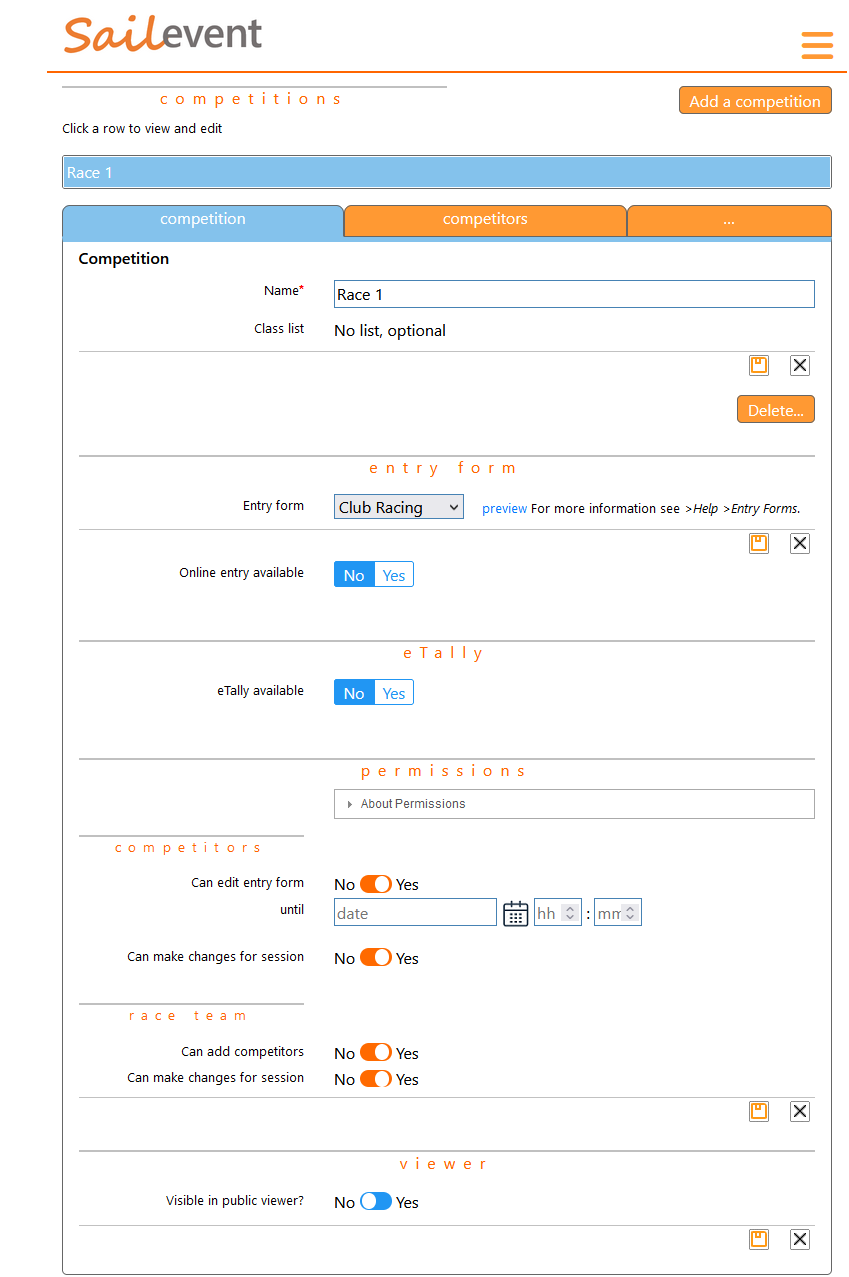
\includegraphics[width=0.6\linewidth]{images/Sailevent.png} 

    \caption{Race creation page in \citet{SailEvent}
    }

    % use the notation fig:name to cross reference a figure
    \label{fig:sailEvent}
\end{figure}


The figure shows the screen of sail event, allowing a club user to create a new race. This differs from its counterpart in \citet{sailwave} as it stays away from the spreadsheet-style of data input, and instead uses a list of different fields. This results in a generally less cluttered look, but makes it harder to understand where and what data input, as a user must take in the whole screen, whereas in \citet{sailwave}, a user must only read the column headers to know what is needed from them.

Due to sail event being a web-app, it has the advantage of being able to be assessed from any device without any set-up, which may suite well to the demographic of Castle Semple Sailing Club, who have limited computer experience to deal with complex setup of software.

\subsection{Summary}

Overall, the good features from the three solutions analysed include:
\begin{itemize}
    \item
    spreadsheet-style data entry from \citet{sailwave}.
    \item
    The simple and stream-lined approach from Sailing Club Manager \citet{ClubManager}.
    \item
    The limited features from and uncluttered look of Sail Event \citet{SailEvent}.
\end{itemize}

The things to stay away from in a new system include:
\begin{itemize}
    \item
    Clutter and bloated-ness of \citet{sailwave} 
    \item
    The wide scope of Sailing \citet{ClubManager}
    \item
    The hard-to-understand user input \citet{SailEvent}
\end{itemize}

All of the examined systems lack something in the context of Castle Semple Sailing Club’s needs, and so there is a gap to bring together the good parts of each of these systems, while keeping close to \citet{sailwave}, as that is what the club is used to, and taking lessons from what these examples did wrong.

\section{Client Meeting}

An initial meeting with the client was held to discuss requirements. It was important to make sure the client’s requirements were correctly identified because, as discussed previously, the client will not be available to regularly check on progress, so there is limited ability to revise the requirements before the system is implemented.  At the meeting, the following requirements were identified:

Main requirements
\begin{itemize}
    \item
    Must be a web-app.
    \item
    Race scored with Portsmouth Yardstick handicap and RYA low scoring rules.
    \item
    people can enter race (entered or do it themselves).
    \item
    people can enter as many or as few races as they like.
    \item
    people can use different boats for each race.
    \item
    like excel spreadsheet but interactive.
    \item
    all can access it to see Leader board.
    \item
    boats are predefined (drop down menu).
\end{itemize}
Extensions
\begin{itemize}
    \item
    discard worst races if you have been in enough.
    \item
    Ability to embed leader board in another website.
    \item
    app to help collect times.
\end{itemize}

\section{Idea Proposals}
From the initial requirements, two general ideas for a system were made.
\subsection{Idea 1}
First is a web-app race manager, very similar to \citet{SailEvent}, with the following features:
\begin{itemize}
    \item
    Admin can create races.
    \item
    sailors can log in to enter themselves into races and view the leader-board.
    \item
    separate accounts for Admin + Sailors.
\end{itemize}

This has the advantage of less work for the person managing races than the current system, as sailors enter themselves, and allows the performance of sailors to be tracked across different series.

However, It does stray a little into complete club management, as all the different accounts would have to be managed. For example, who has access to a sailor account, only those who has paid the club fees? This brings complexity.

\subsection{Idea 2}
An additional idea is a race management program, similar to what the club is already using in \citet{sailwave}, But hosted in a web-app, with a web-app view of the leader-board. This idea takes inspiration from the Victoria park run website \citeyear{Parkrun} where the results are available publicly, but only someone with an admin account can view them. It would have the following features:
\begin{itemize}
    \item
    desktop-style editor with web-app leader-board, all on the web
    \item
    race manager creates races and enters sailors with admin account
    \item
    without admin account, a sailor can only view the leader-board
\end{itemize}

The advantage of the approach is it greatly decrees complexity as no account managing is needed beyond the admin account. However, the approach does have less functionality than idea 1.

\section{The Requirements}
Upon consultation with the client, idea 2 was selected as the best approach. The reduction in complexity, from not having to deal with complex account management, was desirable, as it means the project is more likely to succeeds, with the limited time and
resources available.

Additionally, one of the main problems with the current system, \citep{sailwave}, is that is is complex and bloated with far more features than Castle Semple Sailing Club require. In order to design a new system that improves upon this, it in necessary to strictly limit the features that only that which the club requires. This results in a more lightweight and easy to use system, which is exactly what the current system is not. Removing as much friction as possible in the user's experience is important in this case.

A user stories document was made to summarise the requirements, the contents of which is shown bellow:
\subsection{Minimum Viable Product}
\begin{itemize}
    \item
    Sailor can view the leader-board with a web browser to see who is winning the series.
    \item
    Sailor can view the race results of any race in a series.
    \item
    Race officer can log in to admin account to input information.
    \item
    Race officer can add a new series to start adding races.
    \item
    Race officer can add a sailor to a series so they can enter races.
    \item
    Race officer can add a new race to a series to add race results.
    \item
    Race officer can add a sailor to a race to enter them in the race.
    \item
    Race officer can select which boat the sailor is in to apply
    correct handicap.
    \item
    Race officer can add a sailor’s race time to record a race result.
    \item
    Race officer can remove incorrect sailors, races and series’ to undo mistakes.
    \item
    Race officer can indicate a sailor was a shore officer to give them correct credit.
    \item
    Race officer can indicate a sailor started but didn't finish to give them the correct credit.
    \item
    Race officer can see score of each sailor in the race that is automatically calculated to know the results
    \item
    Race officer can see leader-board automatically updated with scores so that they know the current state of the series
\end{itemize}

\subsection{Should have}

\begin{itemize}
    \item
    A new user can easily install software on their own machine or a cloud platform of their choice to be able to use it.
    \item
    Race officer can define a pattern to exclude worst scoring races if sailor has entered enough of them.
\end{itemize}

\subsection{Could have}
\begin{itemize}
    \item
    A user can embed the leader board of a series in another website to share results easier.
    \item
    Race officer can input race times with an app to make inputting the results in easier.
    \item
    Users can have accounts to track their results across multiple sires.
\end{itemize}

%==================================================================================================================================
\chapter{Design}
The first step in the design is to design a database to store all the necessity information about series races, sailors and boats.
\section{Database}

\begin{figure}[h!]
    \centering
    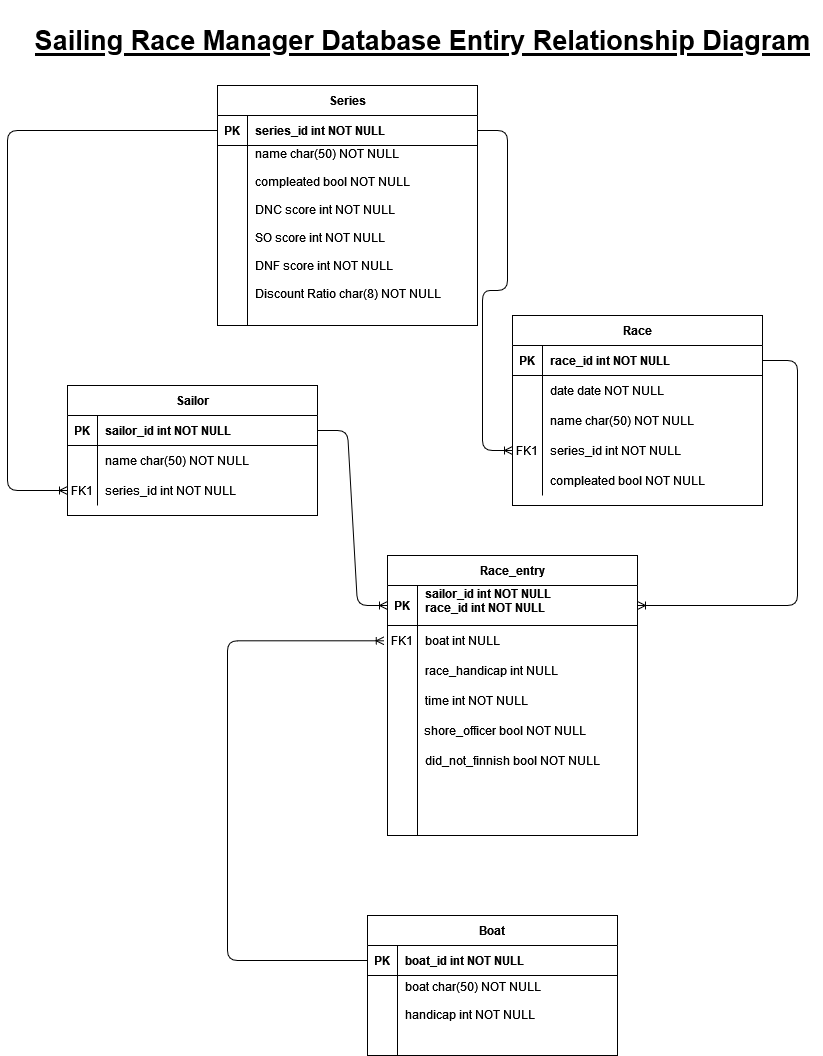
\includegraphics[width=0.7\linewidth]{images/ERD FINAL.png} 

    \caption{Entity Relationship Diagram, showing the different tables in the database, their attributes, and relationships.
    }

    % use the notation fig:name to cross reference a figure
    \label{fig:ERD}
\end{figure}

Figure \ref{fig:ERD} shows an entity relationship diagram of the database. The tables are as follows:
\begin{outline}
    \1
    Series represents a series of races.
        \2
        The name attribute represents the user-entered name of the series. It is up to the user to know which is which in the case of non-unique names.
        \2
        The ongoing attribute represents if the series id still in progress. This should only affect the displaying of the series data.
        \2
        The DNC score attribute (Did not compete) defines the penalty score for not competing in the series. As this is defined per series, it means that different series can have different values for this and the other penalty score attributes, increasing the flexibility of the software.
        \2
        The SO score attribute (Shore officer) defines the penalty score for being a shore officer in a race.
        \2
        The DNF score attribute (Did not finish) defines the penalty score for starting, but not finishing, a race.
        \2
        The discount ratio attribute defines how many races must be competed in for a race score to be discounted. It is saved as a string in the form “N:D”, meaning per N races, discount D races.
    
    \1
    Race represents different races. It is connected to Series by a many-to-one relationship, so that a series can contain multiple races, and a race can be in one series. he attributes of race are quite self-explanatory, apart from the completed attribute, This is similar to the completed attribute in series, representing if a race has had all its results inputted. Only races that are completed are counted towards scoring.
    
    \1
    Sailor represents sailors. A sailor is unique to each series. This is to remove the need to an overall list of all sailors who have every been in a race, and the need to manage this list and keep it up to date. Sailors can be considered on a series by series basis. It also removes all coupling between the series and Sailor tables, so the user can start a new series and not have to worry about any previous data. Because sailors need to be manually entered into each series anyway, having sailors be unique to each series shouldn't require much more effort on the user’s part.
    
    \1
    Boat represents all the boats that can be sailed in a race, along with their Portsmouth Yardstick handicap numbers.
    
    \1
    Race entry represents a sailors entry in a race. It has a composite primary key made up of the Sailor\_id and race\_id attributes, as a race entry is a specific sailor in a specific race.
        \2
        The boat attribute contains the boat that sailor is racing in in that race. Sailors can be in in different boats in different races. This ensures that sailors can only sail in specified boats. It is set to null when a new entry in the table is made.
        \2
        The Race handicap represents the Portsmouth Yardstick (PY) handicap number of the boat at the time of this race. It is copied from the Boat table when the boat is selected. This is done so if the PY number is updated in the future, it does not effect previous races, which will still use the original number stored here.
        \2
        The time attribute contains the raw time the sailor took to complete the race in seconds. It has a default values of 0 when the race is created, which represents a sailor hat did not compete in the race.
        \2
        The corrected time attribute holds the corrected time as calculated by formula \ref{eq:1} previously discussed in chapter \ref{chap:Back}. It is updated whenever any other attribute in the table changes, to always keep it up to date.
        \2
        The shore officer and did not finish attributes indicates reasons why the sailor did not compete in the race that effect score calculation. They have a default value of false on creation.
        \2
        It is assumed that every sailor in a series has a race entry for every race in that series. This is be enforced when new sailors and races are created. There is not attribute for score, as that is be calculated on the fly whenever it is accessed. This removes the possibility of a mismatch between the real score, and the score stored here.
\end{outline}

\section{Site Map}

\begin{figure}[h!]
    \centering
    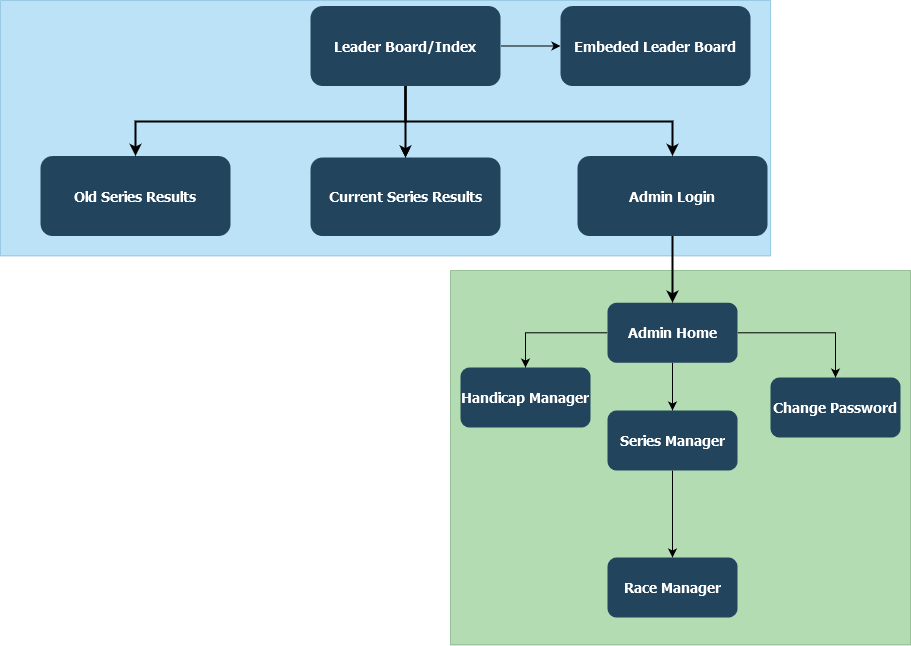
\includegraphics[width=1\linewidth]{images/SiteMap.png} 

    \caption{Site map showing the different pages of the web-app. The coloured boxes clearly show the two different sections of the website.
    }

    % use the notation fig:name to cross reference a figure
    \label{fig:Site Map}
\end{figure}

Figure \ref{fig:Site Map} shows the different pages of the web-app. The coloured boxes around the pages clearly show the two different sections of the website, admin (Blue), and non-admin (Green). Admin in this case means that part of the website that corresponds to the desktop application in \citet{sailwave}. It is only accessible by someone with the admin password, who has the authority to input and edit the results of races. The non-admin section is the one that is available publicly.

\subsection{Non-Admin Section}

\hfill\\
\subsubsection{Leader-board/index page}
\hfill\\
The first page a user sees upon opening the web-app is the leader-board page. This shows a summary of the ongoing series, and lists past series. Figure \ref{fig:LeaderBoardWF} is a wire-frame, showing the design of the page.

\begin{figure}[h!]
    \centering
    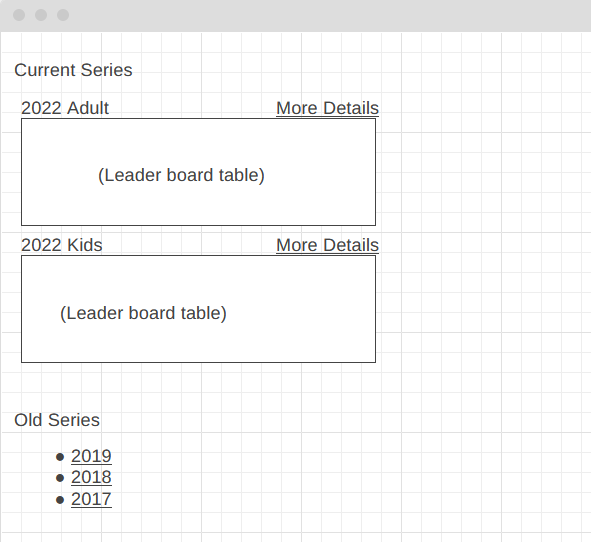
\includegraphics[width=1\linewidth]{images/IndexWireframe.png} 

    \caption{A wire-frame, showing the possible design of the Leader Board page.
    }

    % use the notation fig:name to cross reference a figure
    \label{fig:LeaderBoardWF}
\end{figure}


Series with the competed flag set to false in the database, representing the series that sailors are currently competing in, are displayed first. The leader-board for each series is shown with them.
\begin{itemize}
    \item
    There can be any number of series, as a club may have multiple happening simultaneously, but it is assumed there will be few of them, and so they can all be displayed properly on the same page
    \item
    The total score for each sailor in the Leader-board is not stored in the database, but is calculated from all the scores of all the races in the series. Although this results in more repeated computation on the sever, it removes the possibility of miss-matches between the total score shown and the real score, making adding and updating scores simpler.
    \item
    Each entry contains a link to a results page, showing more detail about the results of the races, including the results of individual races.
\end{itemize}
    
The next section of the page shows the series that have been completed, and a winner declared. The results for these are not as important, so they are hidden separate pages, assessed via links displayed on this page. This reduces clutter while still keeping the information easily accessible to users.

\hfill\\
\subsubsection{Current and old Series results pages}
\hfill\\
These pages show more detail about a specific series. They show the overall series leader-board, and a table for each race that race’s results. Figure \ref{fig:detailsWF} is a wire-frame showing the design:

\begin{figure}[h!]
    \centering
    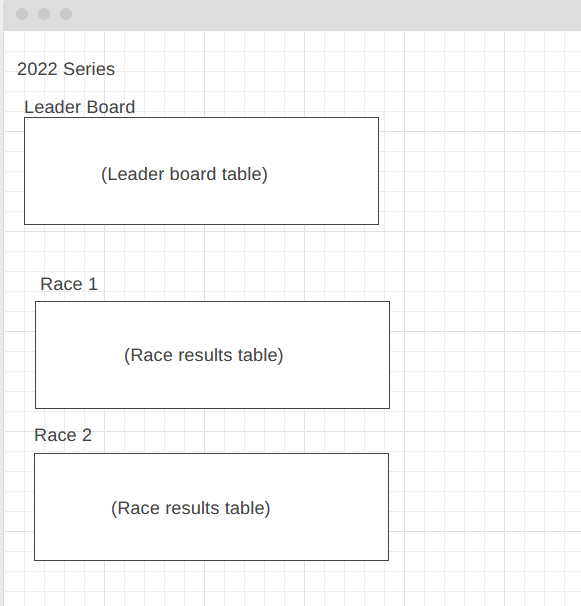
\includegraphics[width=1\linewidth]{images/moreDetailWireframe.png} 

    \caption{A wire-frame, showing the possible design, the current and old series results page.
    }

    % use the notation fig:name to cross reference a figure
    \label{fig:detailsWF}
\end{figure}

\hfill\\
\subsubsection{Embedded Leader-board}
\hfill\\
This page was not in the original design, but was added in later to fulfil the requirement in the could have section of the user stories that: “A user can embed the leader board of a series in another website to share results easier”. The page simply displays the leader-board of a given series, and a user can link this page in their own website to embed the leader-board in it.

\hfill\\
\subsubsection{Admin Login}
\hfill\\
The admin login page is a simple, generic login page that allows the admin user to log in to the admin account, in order to access to admin part of the website. Only a password is required, as there is only one admin account. This was done to reduce the complexity of managing accounts. This account is to be shared amongst all the people at the club responsible for inputting race data, similar to how currently, the single computer with the \citet{sailwave} program is shared.

\subsection{Admin Section}

\hfill\\
\subsubsection{Admin Home}
\hfill\\
This page features a list of all the series as links, split into current and past. Each series links to the series manager page for that series. The user can also use this page to add a new series. The page also contains links to the handicap manager and the change password page. A wire frame of the page is shown in figure \ref{fig:adminHomeWF}.

\begin{figure}[h!]
    \centering
    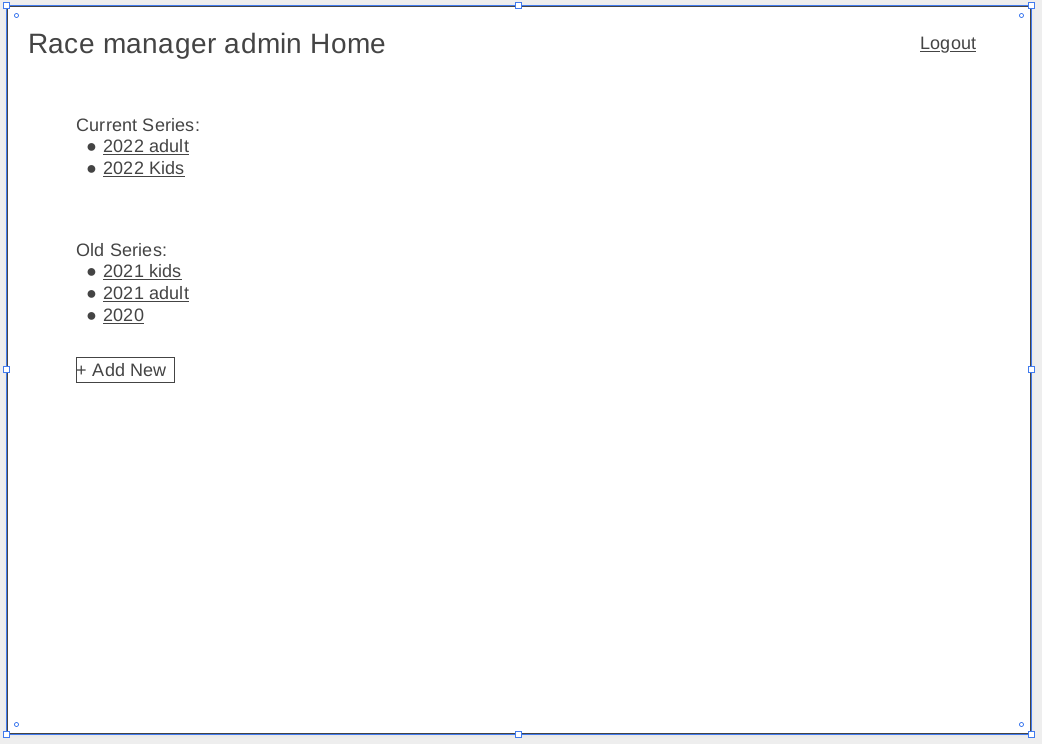
\includegraphics[width=1\linewidth]{images/admin home 2.png} 

    \caption{A wire-frame, showing the possible design of the admin home page.
    }

    % use the notation fig:name to cross reference a figure
    \label{fig:adminHomeWF}
\end{figure}

\hfill\\
\subsubsection{Handicap Manager}
\hfill\\
The handicap manager allows the user to manage a global list of boats and their handicaps. The Portsmouth Yardstick handicap numbers are only available on the RYA website in PDF format. This means that having a system to automatically import the handicap numbers from a file is not feasible, as this is hard to do with a PDF file. Additionally, any solution that did so would be reliant on the format of the Portsmouth Yardstick handicap numbers remaining unchanged.

The best solution that was found was to provide a way for the user to input and update handicap information manually. This also provides the benefit of allowing boats to be used that do not feature in the main Portsmouth Yardstick Scheme. This increases the web-apps flexibility.

The page will consist of an editable table, showing all the boats and handicap numbers currently in the system, with the ability to add more. The software will be delivered to the client with the most up-to-date handicap numbers preinstalled, so less setup is required. It will be up to the client to update thses numbers when new ones are released by the RYA.

\hfill\\
\subsubsection{Change Password}
\hfill\\
This page will feature a simple form allowing the admin user to change the admin password.

\hfill\\
\subsubsection{Series Manager}
\hfill\\
The series manager page allows Admin users to edit a series. This includes adding new races, sailors, editing the parameters such as the penalty scores and the discount ratio and deleting the series. The page will also feature the leader-board for the series, so the user can see the effect of any changes they make. The wire-frame for the page is shown in figure \ref{fig:seriesEditorWF}.

The main features of the page are a couple of editable tables that can be used to add and edit the details of races and sailors. The parameters can be tweaked via a series of options at the top of the page, For example, the completed checkbox in the wire-frame.

\begin{figure}[h!]
    \centering
    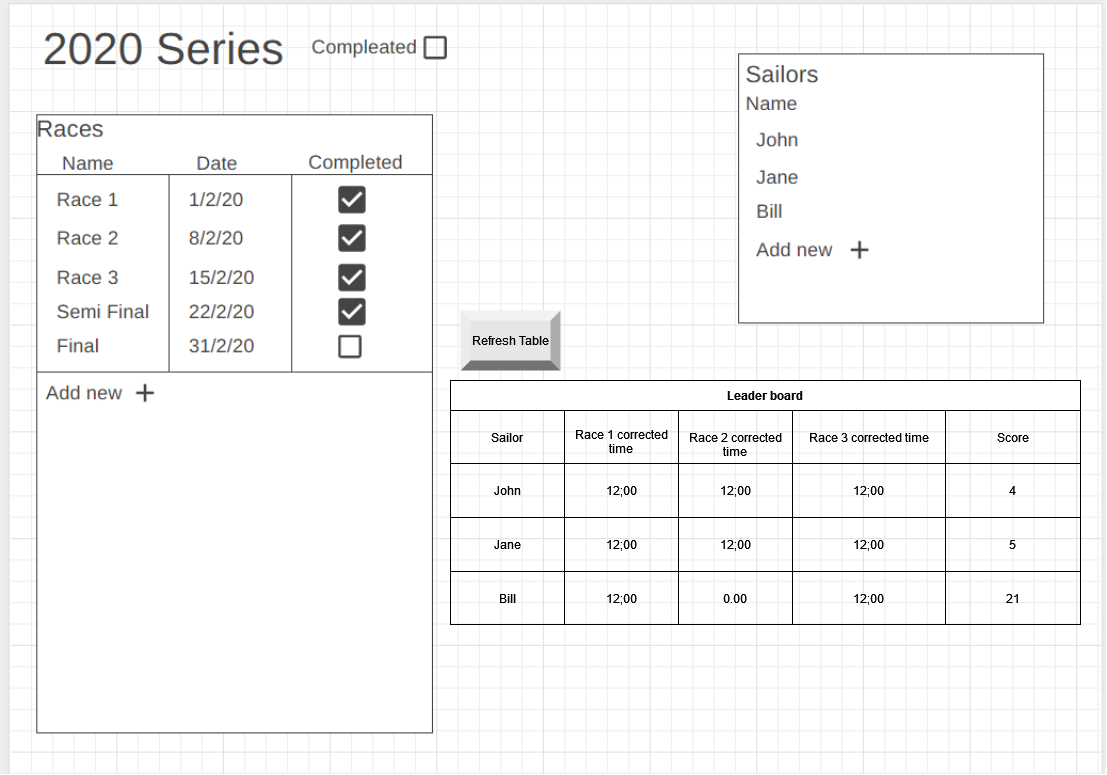
\includegraphics[width=1\linewidth]{images/Series editor 2.png} 

    \caption{A wire-frame, showing a possible design of the series editor page.
    }

    % use the notation fig:name to cross reference a figure
    \label{fig:seriesEditorWF}
\end{figure}

\hfill\\
\subsubsection{Race Manager}
\hfill\\
By clicking on each race, the user is able to open up the race manager page for that race. This is the page where the results for a single race can be entered. Figure \ref{fig:raceEditorWF} is a wire-frame showing a possible design of the race table.

\begin{figure}[h!]
    \centering
    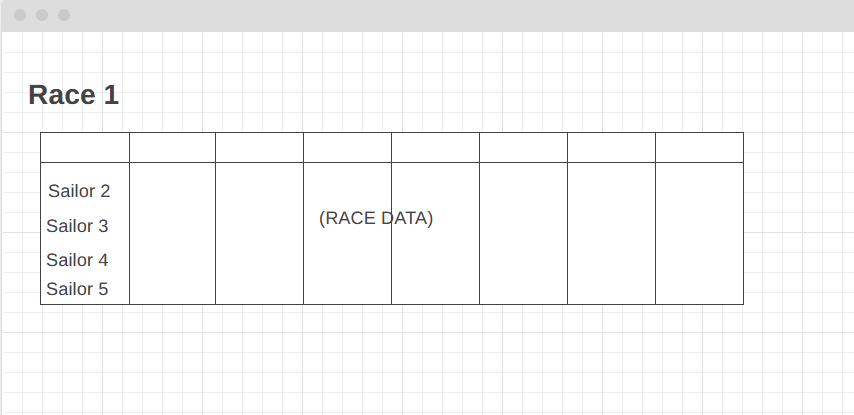
\includegraphics[width=1\linewidth]{images/Race editor.png} 

    \caption{A wire-frame, showing a possible design of the race editor page.
    }

    % use the notation fig:name to cross reference a figure
    \label{fig:raceEditorWF}
\end{figure}

The page mainly features an editable table showing all the race entries for that race. A race entry is a sailor in a race. The fields in the table allow all the database attributes for the Race Entry table to be edited. Unlike the tables on the previous page, the user cannot add new entries manually. Whenever a new race or sailor is added in the series editor, new entries are automatically added to the race entry table. This ensures that there is always a race entry for every sailor in every race. In this way, when a new sailor is added to a series, they are automatically entered into every race in that series. This reduces the workload of the admin user, and ensures that any sailor who didn't complete in a race are counted as not competing, as that is the default sate of a sailor when they are added.

\section{Scoring}

In order to meet the requirements, the web-app must currently process the race data entered by the user into scores.

There are two scores which must be managed, the score for each sailor in a race, and a sailor's total score across a series. One approach would be to store these scores in the Race Entry and Series tables respectively, and update them whenever something changes. However, it was decided that a better approach would be to only calculate the scores when they are needed. While this increases the processing needing to be done on the server, it removes the chance for a mismatch between stored score data, and the inputs. It also reduces the complexity of updating the database, and reduces all the score processing into one algorithm, making it easier to find bugs in it, as there is only a single point of failure.

Formula \ref{eq:1} shown in chapter \ref{chap:Back} will be used to calculate the corrected time from the raw time, whenever an attribute in the Race entry table is updated. When a user loads the Leader Board table, and requests the info from the server, the list of race entries for each race in that series will be sorted by corrected time, and the score for each sailor is calculated via the RYA low scoring race rules \citep{RYAscore}, with penalty scores being awarded where the relevant attributes are set. The scores for every sailor in the series will then be added together, and sorted. They can then be sent to the client-side to be displayed.

In this way, scoring should follow the RYA scoring rules \citep{RYAscore}.

\section{Validation}

The system will be designed to handle as much validation as possible in the database itself so, theoretically, the database cannot be in an invalid state. This means data from the database can be trusted, and so removes the need for extensive validation on data received from the database.

From the point of view of inputting data, where possible, the user will be prevented from entering incorrect data at all. For example, in fields such as time, there only numeric values are valid, the user will not be able to enter non-numeric values at all. This removes the need for lots of validation messages which, especially on a large table with many editable fields that the user may be filling in, could get overwhelming.

\section{Communication with the Database}

The majority of communication with the database will be done on the server-side upon the receipt of a GET for POST request. However, on the pages with editable tables, such as the race editor and Series editor, a different approach is required. In order to avoid having to reload the page every time data in the table is changed by the user, which would be very annoying and may make the site unusable, asynchronous communication with the server in needed. The new data must be sent in a POST request to the server, without reloading the page. From there, the server will update the database.

\section{Conclusion}

Overall, the web-app is designed to be simplistic, and to not crowd pages with too many features, as was the main issue in \citet{sailwave}. The design should meet the requirements, while keeping the interface easy to grasp by non computer skilled users.


%==================================================================================================================================
\chapter{Implementation}
What did you do to implement this idea, and what technical achievements did you make?
\section{Technologies}

\subsection{The Django framework}
This project was developed using the Django web-app framework. This section will explain the Django framework, and discuss why it was chosen

The django webapp

Two web-app frameworks seemed appropriate for this project. Django and flask.

\section{Development methods}

\section{Explanation of implementation}

\section{Evolution of the design}


%==================================================================================================================================
\chapter{Evaluation} 
How good is your solution? How well did you solve the general problem, and what evidence do you have to support that?

\section{Guidance}
\begin{itemize}
    \item
        Ask specific questions that address the general problem.
    \item
        Answer them with precise evidence (graphs, numbers, statistical
        analysis, qualitative analysis).
    \item
        Be fair and be scientific.
    \item
        The key thing is to show that you know how to evaluate your work, not
        that your work is the most amazing product ever.
\end{itemize}

\section{Evidence}
Make sure you present your evidence well. Use appropriate visualisations, reporting techniques and statistical analysis, as appropriate.

If you visualise, follow the basic rules, as illustrated in Figure \ref{fig:boxplot}:
\begin{itemize}
\item Label everything correctly (axis, title, units).
\item Caption thoroughly.
\item Reference in text.
\item \textbf{Include appropriate display of uncertainty (e.g. error bars, Box plot)}
\item Minimize clutter.
\end{itemize}

See the file \texttt{guide\_to\_visualising.pdf} for further information and guidance.

\begin{figure}
    \centering
    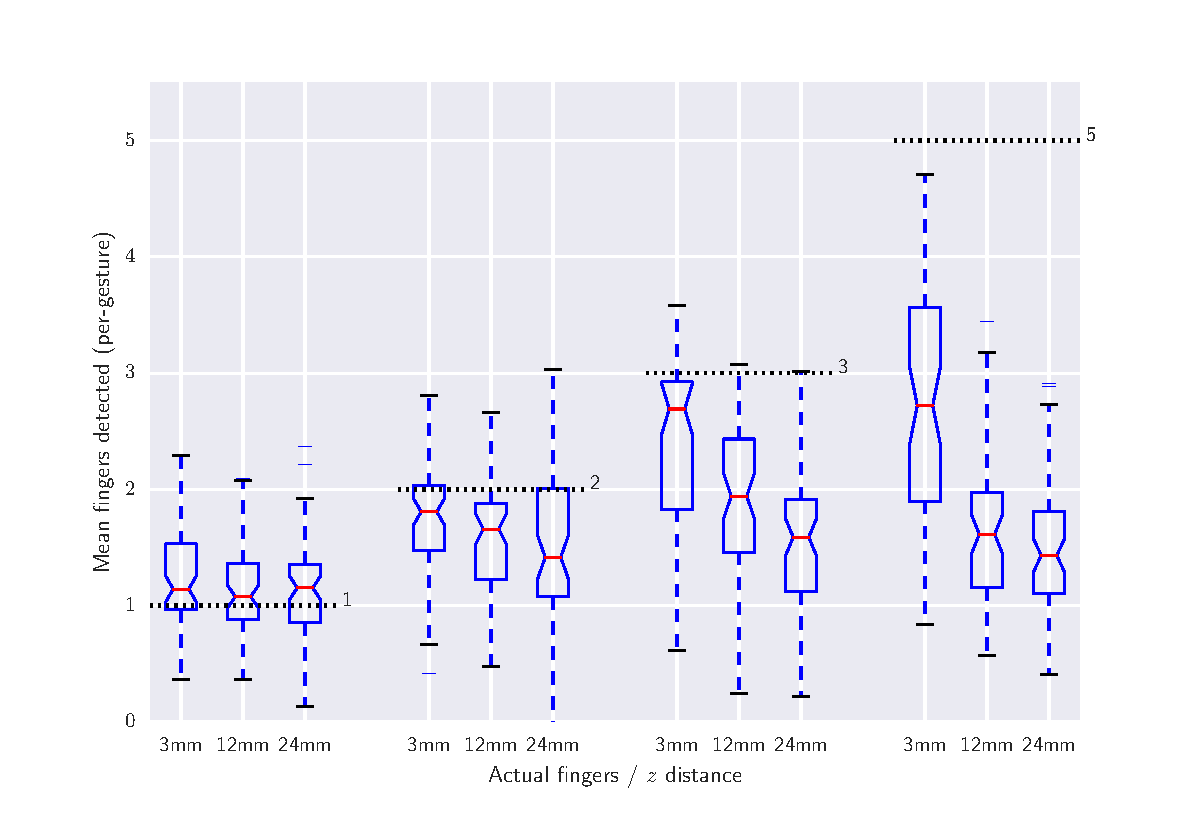
\includegraphics[width=1.0\linewidth]{images/boxplot_finger_distance.pdf}    

    \caption{Average number of fingers detected by the touch sensor at different heights above the surface, averaged over all gestures. Dashed lines indicate
    the true number of fingers present. The Box plots include bootstrapped uncertainty notches for the median. It is clear that the device is biased toward 
    undercounting fingers, particularly at higher $z$ distances.
    }

    % use the notation fig:name to cross reference a figure
    \label{fig:boxplot} 
\end{figure}


%==================================================================================================================================
\chapter{Conclusion}    
Summarise the whole project for a lazy reader who didn't read the rest (e.g. a prize-awarding committee).
\section{Guidance}
\begin{itemize}
    \item
        Summarise briefly and fairly.
    \item
        You should be addressing the general problem you introduced in the
        Introduction.        
    \item
        Include summary of concrete results (``the new compiler ran 2x
        faster'')
    \item
        Indicate what future work could be done, but remember: \textbf{you
        won't get credit for things you haven't done}.
\end{itemize}

%==================================================================================================================================
%
% 
%==================================================================================================================================
%  APPENDICES  

\begin{appendices}

\chapter{Appendices}

Typical inclusions in the appendices are:

\begin{itemize}
\item
  Copies of ethics approvals (required if obtained)
\item
  Copies of questionnaires etc. used to gather data from subjects.
\item
  Extensive tables or figures that are too bulky to fit in the main body of
  the report, particularly ones that are repetitive and summarised in the body.

\item Outline of the source code (e.g. directory structure), or other architecture documentation like class diagrams.

\item User manuals, and any guides to starting/running the software.

\end{itemize}

\textbf{Don't include your source code in the appendices}. It will be
submitted separately.

\end{appendices}

%==================================================================================================================================
%   BIBLIOGRAPHY   

% The bibliography style is abbrvnat
% The bibliography always appears last, after the appendices.

\bibliographystyle{abbrvnat}

\bibliography{l4proj}

\end{document}
